\documentclass[../../main.tex]{subfiles}

\graphicspath{{../../image/}{../../figure/}}

\begin{document}

\section{神经信息传递}\label{section:ch13-神经信息传递}

确保节点标签置换下的不变性或等变性是我们将深度神经网络应用于图结构化数据时的一个关键考虑。另一个关键考量是我们想要利用深度神经网络的表示能力，所以我们保留了“层”的概念，即可以对每一层进行重复的计算变换。如果网络的每一层都在节点重新排序后保持等变性，那么多层叠加后的网络也将保持等变性，同时网络的每一层都受益于图结构信息。

对于输出代表节点级预测的网络，整个网络将按要求表现出等变性。如果网络用来预测图级属性，那么可以在网络的最后添加一个对输入的排列顺序不敏感（置换不变）的层。我们还想确保网络的每一层都是一个高度灵活的非线性函数，并且对其参数具有可微性，以便可以使用自动微分计算梯度，从而通过随机梯度下降进行训练。

图的规模各不相同。例如，不同的分子可以有不同数量的原子，因此标准神经网络使用固定长度表示是不合适的。因此，网络应该能够处理变长输入，正如我们在 Transformer 网络中看到的那样（参见\cref{chapter:ch12-Transformer与注意力机制}）。一些图可能非常大，例如有数百万参与者的社交网络，所以我们也希望构建具有良好扩展性的模型。为了将不变性和等变性内置于网络架构，并促进模型在大型图上的应用，参数共享将发挥重要作用，这一点毋庸置疑。

\subsection{卷积滤波器}\label{subsection:ch13-卷积滤波器}

为了开发符合所有这些要求的框架，我们可以从使用卷积神经网络的图像处理中寻找灵感（参见\cref{chapter:ch10-卷积网络}）。首先我们注意到，图像可以视为图结构化数据的一个特定实例，在这个实例中，节点是像素，边代表图像中相邻的像素对，这里的相邻包括对角相邻的节点以及水平或垂直相邻的节点。

在卷积网络中，我们对图像域进行逐层变换，某个层的一个像素的状态值是由前面层的相关像素的状态值通过计算决定的，用于计算的局部函数称为滤波器（参见\cref{section:ch10-卷积滤波器}）。

\begin{definition}[卷积滤波器]\label{definition:ch13-卷积滤波器}
考虑一个使用 $3\times 3$ 滤波器的卷积层，如\cref{figure:ch13-卷积滤波器图结构}(a)所示。单个的滤波器在第 $(l+1)$ 层的一个像素上执行的计算可以表示为
\begin{align}
z_i^{(l+1)}=f\!\left(\sum_j w_j\,z_j^{(l)}+b\right),
\label{align:ch13-卷积滤波}
\end{align}
其中 $f(\cdot)$ 是一个可微分的非线性激活函数，比如 ReLU 函数，而对 $j$ 的求和则是对第 $l$ 层中一个小块内的所有 $9$ 个像素进行的。相同的函数可以应用于图像中的多个小块，因此权重 $w_j$ 和偏置 $b$ 在各个小块间共享（因此它们不带索引 $i$）。
\end{definition}

% SUPPLEMENT: parent=definition:ch13-卷积滤波器; kind=motivation; location=紧随其后的 remark（重构新增）
\begin{remark}（重构新增）
\eqref{align:ch13-卷积滤波}中有两点是后面推广的起点。其一是求和指标 $j$ 的取值范围：它不是全部像素，而只是与像素 $i$ 相邻的那 $9$ 个位置，这个范围由图像网格的邻接关系决定，换成一般的图就变成 $\mathcal{N}(i)$。其二是参数不带位置索引：$w_j$ 对所有小块相同，因而全部像素共享同一组权重。正是这一共享使参数量与图像大小无关，也使\eqref{align:ch13-卷积滤波}的卷积层具有平移等变性。\par
需要区分 $w_j$ 的下标 $j$ 与节点的下标：$j$ 枚举的是一个 $3\times 3$ 小块内部的相对位置，它共有 $9$ 个取值，与图像中有多少个像素无关；而 $i$ 枚举的是像素。正因为这两类索引的性质不同，\eqref{align:ch13-卷积滤波}才可能在节点重排下失效——重排节点会打乱“相对位置”与“权重分量”的对应，而权重向量本身并没有随之重排。这一观察直接引出下面的图形式改写。
\end{remark}

\begin{figure}[htbp]
  \centering
  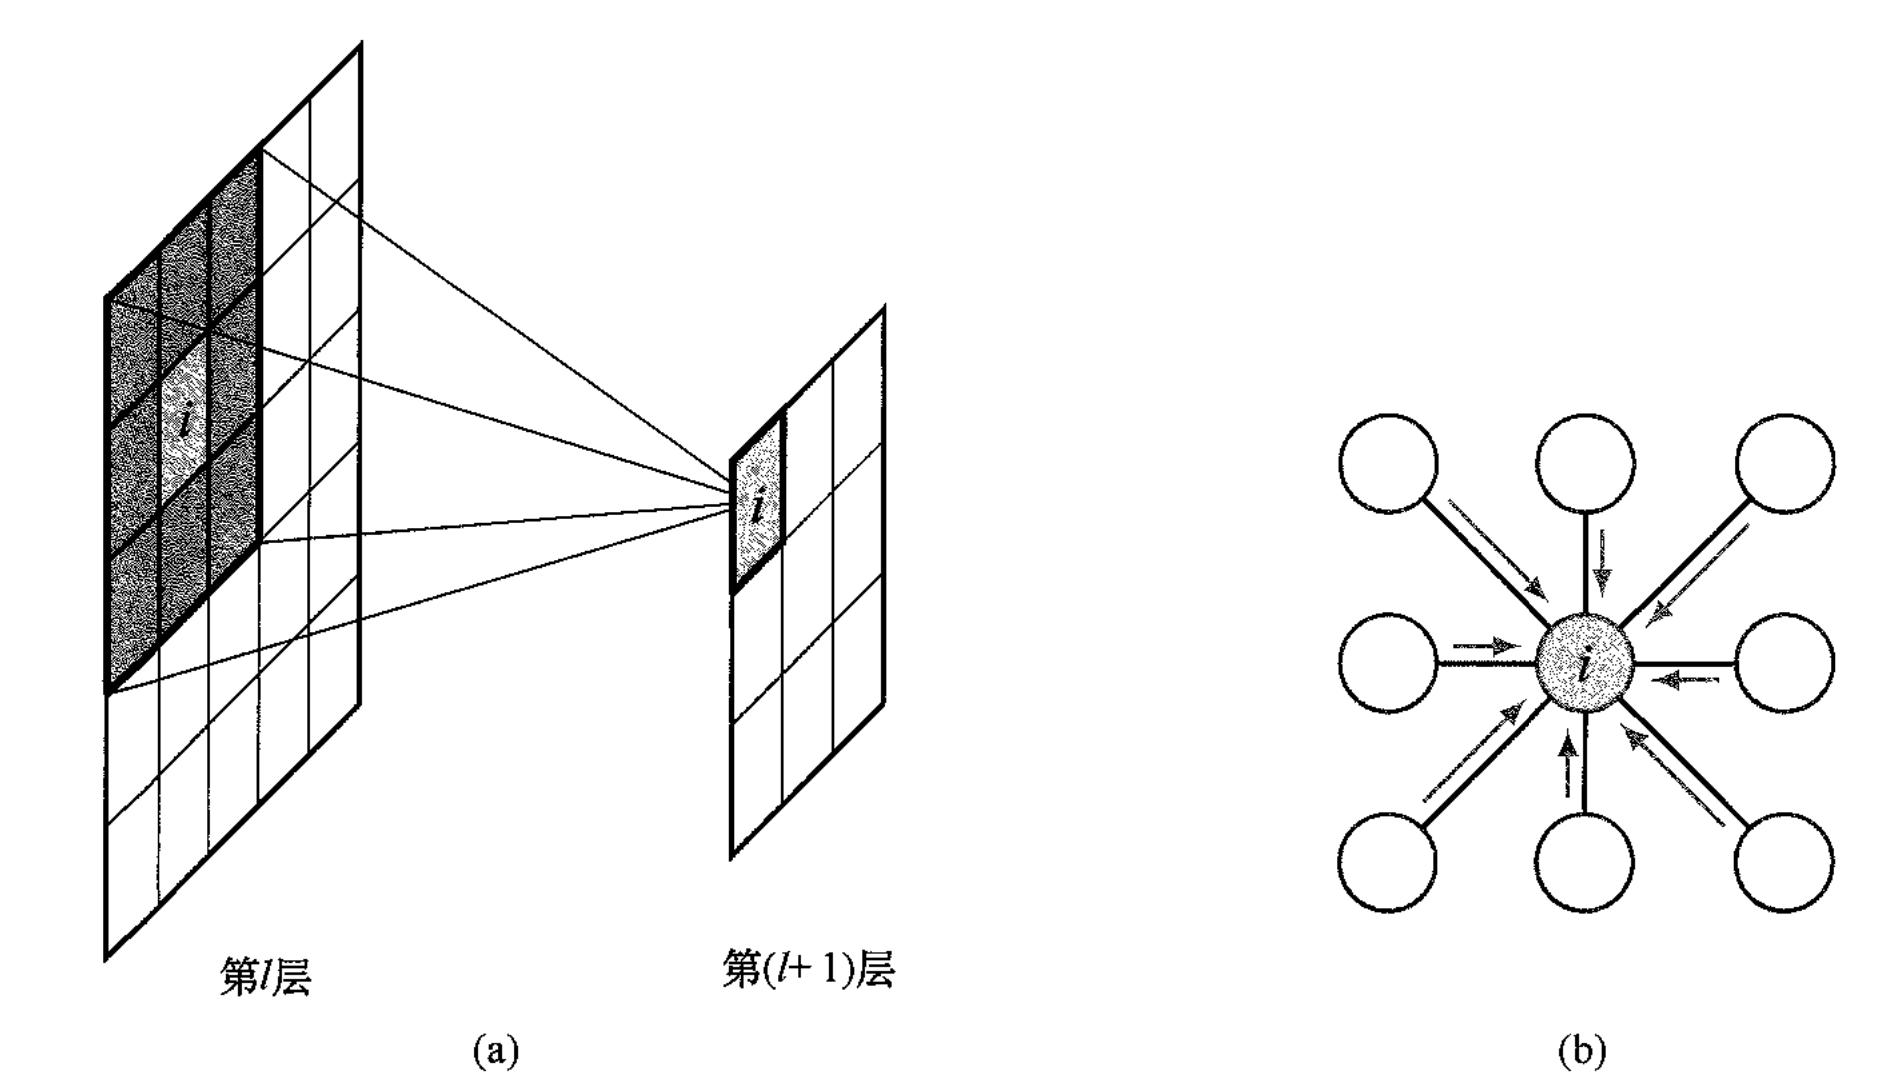
\includegraphics[width=0.85\textwidth]{ch13-fig13.3-conv-graph.png}
  \caption{图像的卷积滤波器可以表示为一种图结构计算：(a) 在深度卷积网络的第 $(l+1)$ 层，节点 $i$ 的值是由第 $l$ 层局部像素区域激活值通过滤波器函数计算得来的；(b) 将同样的计算结构以图的形式表达，“消息”从节点 $i$ 的邻居节点流向节点 $i$}
  \label{figure:ch13-卷积滤波器图结构}
\end{figure}

\eqref{align:ch13-卷积滤波}在第 $l$ 层节点置换下不是等变的，因为权重向量中的 $w_j$ 元素在排列上不是不变的。然而，我们可以通过进行一些简单的修改来实现等变性，具体步骤如下。首先将滤波器视为一个图，如\cref{figure:ch13-卷积滤波器图结构}(b)所示，并且从中分离出来自节点 $i$ 的贡献。其他 $8$ 个节点构成节点 $i$ 的邻居节点集合 $\mathcal{N}(i)$。

\begin{definition}[图形式的卷积滤波器]\label{definition:ch13-图形式卷积滤波器}
假设单个权重参数 $w_{\mathrm{neigh}}$ 在邻居节点间共享，则图形式的卷积滤波器定义为
\begin{align}
z_i^{(l+1)}=f\!\left(w_{\mathrm{neigh}}\sum_{j\in\mathcal{N}(i)}z_j^{(l)}+w_{\mathrm{self}}\,z_i^{(l)}+b\right),
\label{align:ch13-图卷积滤波}
\end{align}
其中节点 $i$ 有自己的权重参数 $w_{\mathrm{self}}$。
\end{definition}

% SUPPLEMENT: parent=definition:ch13-图形式卷积滤波器; kind=motivation; location=紧随其后的 remark（重构新增）
\begin{remark}（重构新增）
\eqref{align:ch13-图卷积滤波}相对\eqref{align:ch13-卷积滤波}只做了两处改动，但这两处改动的地位并不相同。第一处是把“$3\times 3$ 小块内按相对位置编号的 $9$ 个权重 $w_j$”换成“邻居共用的一个标量 $w_{\mathrm{neigh}}$”：这消除了权重分量与邻居编号之间的对应关系，是获得等变性的关键。第二处是把节点自身从求和中分离出来，单独乘以 $w_{\mathrm{self}}$：这一步与等变性无关，它只是补回了“中心像素与邻居地位不同”这一信息，否则中心节点与邻居将无法区分。\par
代价也必须说清楚：单个 $w_{\mathrm{neigh}}$ 的表达能力弱于 $9$ 个独立的 $w_j$，因为卷积层原本可以利用“上、下、左、右”等方向差异，而图形式的滤波器把所有邻居一视同仁。这正是为什么后续要引入对邻居嵌入先做变换的聚合算子（\eqref{align:ch13-深度集合聚合}）：用共享的 $\operatorname{MLP}_\phi$ 恢复表达力，同时不破坏对称性。\par
系数 $w_{\mathrm{neigh}}$、$w_{\mathrm{self}}$ 与偏置 $b$ 必须在全部节点间共享；若允许每个节点有自己的参数，等变性立刻失效，因为重排节点会改变“哪个参数属于哪个节点”。
\end{remark}

\begin{proposition}[图形式卷积滤波器的置换等变性]\label{proposition:ch13-图滤波器等变性}
设 $\bm{z}^{(l)}=(z_1^{(l)},\cdots,z_N^{(l)})^{\mathsf T}$ 为第 $l$ 层的激活向量，$\bm{P}$ 为任意 $N\times N$ 置换矩阵，$\widetilde{\bm{z}}^{(l)}=\bm{P}\bm{z}^{(l)}$，并记 $\widetilde{\mathcal{N}}(i)$ 为按 $\bm{P}$ 重排后的邻居集合。则按\eqref{align:ch13-图卷积滤波}逐节点计算得到的第 $(l+1)$ 层激活满足
\begin{align*}
\widetilde{\bm{z}}^{(l+1)}=\bm{P}\bm{z}^{(l+1)}.
\end{align*}
\end{proposition}

\begin{proof}
我们可以将\eqref{align:ch13-图卷积滤波}解释为通过从邻居节点收集信息来更新节点 $i$ 处的局部表示 $z_i$，这通过从邻居节点传递给节点 $i$ 的消息来实现。在这种情况下，消息直接是其他节点的激活状态。随后将这些消息与节点 $i$ 的信息结合，并使用非线性函数进行转换。来自邻居节点的信息通过\eqref{align:ch13-图卷积滤波}中的简单求和聚合起来，这显然对于与这些节点相关联的标签的任何排列都是不变的。将以上操作同步应用于图中的每个节点，因此如果节点被排序，则最终的计算将保持不变，但它们也将被相应地置换，因此这个计算在节点重新排序下是等变的。
把上述论证写成指标形式：重排之后，编号为 $i$ 的节点实际上就是原来的节点 $\pi^{-1}(i)$，于是它的邻居集合为 $\widetilde{\mathcal{N}}(i)=\pi\big(\mathcal{N}(\pi^{-1}(i))\big)$，而 $\widetilde z_j^{(l)}=z_{\pi^{-1}(j)}^{(l)}$。代入\eqref{align:ch13-图卷积滤波}得
\begin{align*}
\widetilde z_i^{(l+1)}&=f\!\left(w_{\mathrm{neigh}}\sum_{j\in\widetilde{\mathcal{N}}(i)}\widetilde z_j^{(l)}+w_{\mathrm{self}}\widetilde z_i^{(l)}+b\right)\\
&=f\!\left(w_{\mathrm{neigh}}\sum_{j'\in\mathcal{N}(\pi^{-1}(i))}z_{j'}^{(l)}+w_{\mathrm{self}}z_{\pi^{-1}(i)}^{(l)}+b\right)=z_{\pi^{-1}(i)}^{(l+1)}.
\end{align*}
第二个等号只是把求和变量由 $j\in\widetilde{\mathcal{N}}(i)$ 换成 $j'=\pi^{-1}(j)\in\mathcal{N}(\pi^{-1}(i))$，这是有限集合上的重指标，不改变求和值；$w_{\mathrm{neigh}}$、$w_{\mathrm{self}}$、$b$ 与 $i$ 无关，故可原样保留。最后一式表明 $\widetilde{\bm{z}}^{(l+1)}$ 的第 $i$ 个分量等于 $\bm{z}^{(l+1)}$ 的第 $\pi^{-1}(i)$ 个分量，即 $\widetilde{\bm{z}}^{(l+1)}=\bm{P}\bm{z}^{(l+1)}$。证毕。
\end{proof}

% SUPPLEMENT: parent=proposition:ch13-图滤波器等变性; kind=motivation; location=紧随其后的 remark（重构新增）
\begin{remark}（重构新增）
这条命题把“卷积可以写成图上的消息传递而不破坏对称性”这句话变成了可检验的等式，它的使用条件是三条：求和只遍历邻居集合、每个邻居的贡献只通过同一个标量 $w_{\mathrm{neigh}}$ 进入、非线性函数 $f$ 逐元素作用。第三条容易被忽略：若 $f$ 依赖分量的位置（例如对向量做固定的线性混合），等变性就不再成立。\par
注意命题只断言等变性，没有断言不变性。$z_i$ 本身会随节点重排而换位，这是节点级量的正确行为；若要得到图级的不变量，还需在最后对全部节点做一次置换不变的聚合，这正是\cref{subsection:ch13-图分类}的内容。\par
最后，本命题讨论的是标量激活 $z_n$，它只是下一节向量值嵌入 $\bm{h}_n$ 的一维特例；一般情形见\cref{theorem:ch13-图网络等变性}。
\end{remark}

\subsection{图卷积网络}\label{subsection:ch13-图卷积网络}

我们以卷积操作为例，构建用于处理图结构数据的深度神经网络模型。我们的目标是定义一种灵活的、非线性的节点嵌入转换，它对一组权重和偏置参数可微分，并且将第 $l$ 层中的变量映射到第 $(l+1)$ 层的相应变量。

\begin{definition}[节点嵌入]\label{definition:ch13-节点嵌入}
对于图中的每个节点 $n$ 以及网络中的每一层 $l$，引入一个 $D$ 维的列向量 $\bm{h}_n^{(l)}$ 作为节点嵌入变量，其中 $n=1,\cdots,N$ 且 $l=1,\cdots,L$。
\end{definition}

% SUPPLEMENT: parent=definition:ch13-节点嵌入; kind=motivation; location=紧随其后的 remark（重构新增）
\begin{remark}（重构新增）
节点嵌入是“把结构信息写进特征”的载体：$\bm{h}_n^{(l)}$ 的第 $l$ 层版本应当同时编码节点 $n$ 自身的属性与它 $l$ 跳邻域内的结构。因此 $\bm{h}_n^{(l)}$ 的维数 $D$ 是一个建模选择，它不必等于输入特征维数——\eqref{align:ch13-更新算子}之后的初始化讨论给出了三种把 $\bm{x}_n$ 变成合适维数的方法。\par
上标 $(l)$ 不是幂次而是层号，这一点在\eqref{align:ch13-层叠}中尤其要注意：那里 $\bm{H}^{(l)}$ 表示第 $l$ 层的整块嵌入矩阵。层号从 $0$ 开始计（$\bm{h}_n^{(0)}=\bm{x}_n$），而层的变换共 $L$ 次，因此最终的表示是 $\bm{h}_n^{(L)}$。
\end{remark}

\eqref{align:ch13-图卷积滤波}给出的转换首先从邻居节点收集和合并信息，然后用当前节点嵌入和传入消息的函数更新节点。因此，我们可以将每一层的处理视为两个连续阶段。首先是聚合阶段，对于每个节点 $n$，将消息从其邻居节点传递到该节点，并以置换不变的方式组合成一个新的向量 $\bm{z}_n^{(l)}$。然后是更新阶段，将邻居节点的聚合信息与节点本身的局部信息结合，计算出该节点更新后的嵌入向量。

\begin{definition}[消息传递神经网络]\label{definition:ch13-消息传递神经网络}
考虑图中的一个特定节点 $n$。首先聚合来自节点 $n$ 的所有邻居节点的节点向量：
\begin{align}
\bm{z}_n^{(l)}=\operatorname{Aggregate}\!\left(\{\bm{h}_m^{(l)}:m\in\mathcal{N}(n)\}\right).
\label{align:ch13-聚合定义}
\end{align}
如果聚合函数对变化的邻居节点数量有良好的定义，并且不依赖于这些节点的排序，那么该聚合函数的形式将非常灵活。只要它是一个对这些参数可微分的函数，便于进行梯度下降训练，它就可以包含可学习参数。然后使用另一种操作来更新节点 $n$ 处的嵌入向量：
\begin{align}
\bm{h}_n^{(l+1)}=\operatorname{Update}\!\left(\bm{h}_n^{(l)},\bm{z}_n^{(l)}\right).
\label{align:ch13-更新定义}
\end{align}
同样，这可以是一组可学习参数的可微分函数。并行地对图中的每个节点执行聚合操作，然后执行更新操作。节点嵌入通常使用观测到的节点数据初始化，因此 $\bm{h}_n^{(0)}=\bm{x}_n$。注意，每一层通常都有自己的参数，尽管参数也可以跨层共享。这个框架称为消息传递神经网络（message-passing neural network）（Gilmer et al., 2017），算法 13.1 对它做了总结。
\end{definition}

% SUPPLEMENT: parent=definition:ch13-消息传递神经网络; kind=motivation; location=紧随其后的 remark（重构新增）
\begin{remark}（重构新增）
这个定义把“一层图神经网络”拆成两个可以分别设计的部件，其意义在于：置换等变性只由聚合函数决定，而表达能力主要由更新函数决定。具体地说，$\operatorname{Aggregate}$ 的输入是一个集合 $\{\bm{h}_m^{(l)}:m\in\mathcal{N}(n)\}$，集合本身没有顺序，因此任何以集合为定义域的函数自动是置换不变的；而 $\operatorname{Update}$ 的输入是一个有序对 $(\bm{h}_n^{(l)},\bm{z}_n^{(l)})$，它逐节点作用、参数共享，因此保持等变性（\cref{theorem:ch13-图网络等变性}）。\par
定义中的三个条件缺一不可。第一，“对变化的邻居节点数量有良好的定义”排除了把邻居向量拼接成定长向量的做法——那样一旦度数改变，输入维数就变了。第二，“不依赖于这些节点的排序”排除了带位置索引的加权求和。第三，“对参数可微分”保证梯度可以通过 $\operatorname{Aggregate}$ 与 $\operatorname{Update}$ 反传，这是整个框架能用随机梯度下降训练的前提。注意可学习参数是允许的，被禁止的只是对顺序的依赖。\par
$\bm{h}_n^{(0)}=\bm{x}_n$ 只是最常用的初始化；当 $\bm{x}_n$ 的维数与所需的 $D$ 不同，或节点根本没有观测数据时，需要另作处理（见\eqref{align:ch13-简单更新}之后的讨论）。
\end{remark}

\begin{center}
\fbox{\begin{minipage}{0.9\textwidth}
\small
\textbf{算法 13.1：一个简单的消息传递神经网络}\par\smallskip
\textbf{输入：}无向图 $\mathcal{G}=(\mathcal{V},\mathcal{E})$；初始节点嵌入 $\{\bm{h}_n^{(0)}=\bm{x}_n\}$；聚合函数 $\operatorname{Aggregate}(\cdot)$；更新函数 $\operatorname{Update}(\cdot,\cdot)$\par
\textbf{输出：}最终节点嵌入 $\{\bm{h}_n^{(L)}\}$\par
\smallskip
\hrule\smallskip
\emph{// 迭代进行消息传递}\\
\textbf{for} $l\in\{0,\cdots,L-1\}$ \textbf{do}\\
\hspace*{2em}$\bm{z}_n^{(l)}\leftarrow\operatorname{Aggregate}\left(\{\bm{h}_m^{(l)}:m\in\mathcal{N}(n)\}\right)$\\
\hspace*{2em}$\bm{h}_n^{(l+1)}\leftarrow\operatorname{Update}\left(\bm{h}_n^{(l)},\bm{z}_n^{(l)}\right)$\\
\textbf{end for}\\
\textbf{return} $\{\bm{h}_n^{(L)}\}$
\end{minipage}}
\end{center}

\subsection{聚合算子}\label{subsection:ch13-聚合算子}

聚合函数有许多可能的形式，但它必须仅依赖于输入的集合，而不依赖于输入的顺序。它还必须是任何可学习参数的可微分函数。

\begin{definition}[聚合算子]\label{definition:ch13-聚合算子}
根据\eqref{align:ch13-图卷积滤波}，最简单的聚合函数为求和
\begin{align}
\operatorname{Aggregate}\!\left(\{\bm{h}_m^{(l)}:m\in\mathcal{N}(n)\}\right)=\sum_{m\in\mathcal{N}(n)}\bm{h}_m^{(l)}.
\label{align:ch13-求和聚合}
\end{align}
简单求和显然独立于邻居节点的排序，并且无论邻居节点集合中有多少节点，它都是明确定义的。注意这里没有可学习参数。
\end{definition}

% SUPPLEMENT: parent=definition:ch13-聚合算子; kind=motivation; location=紧随其后的 remark（重构新增）
\begin{remark}（重构新增）
求和之所以是“最简单”的聚合，是因为它在所有置换不变的算子中形式最简，并且同时满足三条要求：对邻居集合的排序不变、对邻居个数不设上限、且与线性变换可交换（$\sum_m\bm{W}\bm{h}_m=\bm{W}\sum_m\bm{h}_m$）。最后一条尤其重要——由于 $\sum_m\bm{h}_m$ 是线性的，\eqref{align:ch13-图卷积聚合}与\eqref{align:ch13-深度集合聚合}中“先变换再求和”与“先求和再变换”只差一个矩阵乘法次序，这使整层可以写成矩阵形式（见\cref{exercise:ch13-06}）。\par
但求和也有明确的缺陷：它的数值随度数增长。一个度为 $10^4$ 的节点，其聚合量的量级会比度为 $1$ 的节点大四个数量级，训练时容易造成梯度尺度失衡。\eqref{align:ch13-平均聚合}与\eqref{align:ch13-图卷积聚合}都是针对这一点做的修正，代价各不相同。\par
定义中“没有可学习参数”不是缺陷而是特性：它保证聚合本身不会破坏对称性。可学习参数应当放在逐节点共享的变换里（\eqref{align:ch13-深度集合聚合}），而不是放在对邻居的加权里——后者若权重依赖邻居的编号就会破坏等变性，若权重依赖邻居的特征则变成注意力（\cref{subsection:ch13-图注意力网络}）。
\end{remark}

相对于那些邻居节点较少的节点，拥有众多邻居的节点会被求和操作赋予更强的影响力，这可能导致数值计算问题，特别是在像社交网络这样的应用中，邻居节点集合的大小可能会相差好几个数量级。这种方法的一个变体是将聚合操作定义为邻居嵌入向量的平均值，即
\begin{align}
\operatorname{Aggregate}\!\left(\{\bm{h}_m^{(l)}:m\in\mathcal{N}(n)\}\right)=\frac{1}{|\mathcal{N}(n)|}\sum_{m\in\mathcal{N}(n)}\bm{h}_m^{(l)},
\label{align:ch13-平均聚合}
\end{align}
其中 $|\mathcal{N}(n)|$ 表示邻居节点集合 $\mathcal{N}(n)$ 中的节点数量。然而，这种归一化抛弃了关于网络结构的信息，并且被证明比简单的求和（Hamilton, 2020）要弱，因此是否使用它取决于节点特征和图结构相比谁更重要。

这种方法的另一个变体（Kipf and Welling, 2016）则考虑到了每个节点的邻居的数量：
\begin{align}
\operatorname{Aggregate}\!\left(\{\bm{h}_m^{(l)}:m\in\mathcal{N}(n)\}\right)=\sum_{m\in\mathcal{N}(n)}\frac{\bm{h}_m^{(l)}}{\sqrt{|\mathcal{N}(n)|\,|\mathcal{N}(m)|}}.
\label{align:ch13-图卷积聚合}
\end{align}

最后一种可能性是取邻居嵌入向量的逐元素最大值（或最小值），这同样满足所需特性，即对数量可变的邻居节点能作出良好定义，并且和邻居节点顺序无关。

\begin{proposition}[图卷积聚合的谱解释（重构新增）]\label{proposition:ch13-图卷积谱解释}
% SUPPLEMENT: parent=align:ch13-图卷积聚合; kind=motivation
设 $\bm{D}\triangleq\operatorname{diag}(d_1,\cdots,d_N)$ 为度矩阵，其中 $d_n=|\mathcal{N}(n)|>0$，$\bm{A}$ 为邻接矩阵，$\bm{H}\in\mathbb{R}^{N\times D}$ 的第 $n$ 行为 $\bm{h}_n^{\mathsf T}$。则\eqref{align:ch13-图卷积聚合}给出的聚合量的转置恰为对称归一化矩阵 $\widehat{\bm{A}}\triangleq\bm{D}^{-1/2}\bm{A}\bm{D}^{-1/2}$ 所作用的结果，即整层可以写成
\begin{align*}
\bm{Z}=\widehat{\bm{A}}\bm{H}=\bm{D}^{-1/2}\bm{A}\bm{D}^{-1/2}\bm{H}.
\end{align*}
特别地，$\widehat{\bm{A}}=\bm{I}-\bm{L}_{\mathrm{sym}}$，其中 $\bm{L}_{\mathrm{sym}}\triangleq\bm{I}-\bm{D}^{-1/2}\bm{A}\bm{D}^{-1/2}$ 是对称归一化 Laplacian。
\end{proposition}

\begin{proof}（重构新增）
按矩阵乘法展开，$\widehat{\bm{A}}$ 的 $(n,m)$ 元为
\begin{align*}
\widehat{A}_{nm}=\left(\bm{D}^{-1/2}\right)_{nn}A_{nm}\left(\bm{D}^{-1/2}\right)_{mm}=\frac{A_{nm}}{\sqrt{d_n d_m}}.
\end{align*}
于是 $(\widehat{\bm{A}}\bm{H})$ 的第 $n$ 行为
\begin{align*}
\left(\widehat{\bm{A}}\bm{H}\right)_{n:}=\sum_{m=1}^{N}\widehat{A}_{nm}\bm{h}_m^{\mathsf T}=\sum_{m\in\mathcal{N}(n)}\frac{\bm{h}_m^{\mathsf T}}{\sqrt{d_n d_m}},
\end{align*}
其中第二个等号用到 $A_{nm}=1$ 当且仅当 $m\in\mathcal{N}(n)$。这正是\eqref{align:ch13-图卷积聚合}的右端（取转置），故 $\bm{Z}=\widehat{\bm{A}}\bm{H}$。又因 $\bm{L}_{\mathrm{sym}}=\bm{I}-\bm{D}^{-1/2}\bm{A}\bm{D}^{-1/2}$ 逐项相减即得 $\widehat{\bm{A}}=\bm{I}-\bm{L}_{\mathrm{sym}}$。
由于 $\bm{A}$ 对称、$\bm{D}$ 为对角正定矩阵，$\bm{L}_{\mathrm{sym}}$ 是对称半正定矩阵，故存在正交矩阵 $\bm{U}$ 与对角矩阵 $\bm{\Lambda}=\operatorname{diag}(\lambda_1,\cdots,\lambda_N)$ 使 $\bm{L}_{\mathrm{sym}}=\bm{U}\bm{\Lambda}\bm{U}^{\mathsf T}$，于是
\begin{align*}
\bm{Z}=\bm{U}\left(\bm{I}-\bm{\Lambda}\right)\bm{U}^{\mathsf T}\bm{H},
\end{align*}
即该聚合层在 $\bm{L}_{\mathrm{sym}}$ 的特征基下对节点特征逐模态地乘以响应 $1-\lambda_i$。证毕。
\end{proof}

% SUPPLEMENT: parent=proposition:ch13-图卷积谱解释; kind=motivation; location=紧随其后的 remark（重构新增）
\begin{remark}（重构新增）
这条命题补出的是原书仅以文献引用带过的 Kipf and Welling (2016) 归一化的矩阵含义：\eqref{align:ch13-图卷积聚合}的分母 $\sqrt{|\mathcal{N}(n)|\,|\mathcal{N}(m)|}$ 不是随手选的缩放，它恰好使聚合算子成为一个对称矩阵 $\widehat{\bm{A}}$ 的乘法。对称性带来两个直接后果：$\widehat{\bm{A}}$ 可正交对角化，从而上一段的谱分解成立；$\widehat{\bm{A}}$ 的特征值落在 $[-1,1]$ 内，反复相乘不会指数爆炸，这正是深堆叠图卷积比直接使用 $\bm{A}$ 更稳定的原因。\par
与\eqref{align:ch13-平均聚合}比较可以看出归一化的两种取舍：平均按行归一，只消除度数对量级的影响，得到的是非对称算子 $\bm{D}^{-1}\bm{A}$；对称归一同时按行与列缩放，保留了 $\bm{A}$ 的对称性因而保留了谱结构。原书说“平均化抛弃了网络结构的信息”，在矩阵语言里就是 $\bm{D}^{-1}\bm{A}$ 与 $\bm{A}$ 不再相似，其特征值不再直接反映图的结构。\par
需要指出，谱解释只是理解该算子的一种视角：它把一次聚合看作一次固定的低通滤波，滤波器形状由 $1-\lambda_i$ 决定，其中不含可学习参数。原书并未展开这一视角，本命题与证明属于重构新增内容。$\bm{D}$ 可逆（即每个节点至少有一个邻居）是本命题的前提；孤立节点会使 $d_n=0$，此时两种归一化都无定义，实际实现中通常给孤立节点补一个自环。
\end{remark}

图神经网络中给定层的每个节点通过聚合前一层的邻居节点信息来更新，这就出现了感受野（receptive field）的概念，类似于\cref{chapter:ch10-卷积网络}中 CNN 所使用的滤波器的感受野（见\cref{definition:ch10-感受野}）。随着信息通过连续的层被处理，对当前层某个节点的更新就会依赖于越来越多的早期层的其他节点，直到有效的感受野几乎覆盖整个图为止，如\cref{figure:ch13-感受野}所示。然而，大的稀疏图可能需要非常多的层，才能使每个输出受每个输入的影响。因此，有些架构引入了一个额外的“超级节点”，它直接连接到原始图中的每个节点，使信息得到快速传播。

\begin{figure}[htbp]
  \centering
  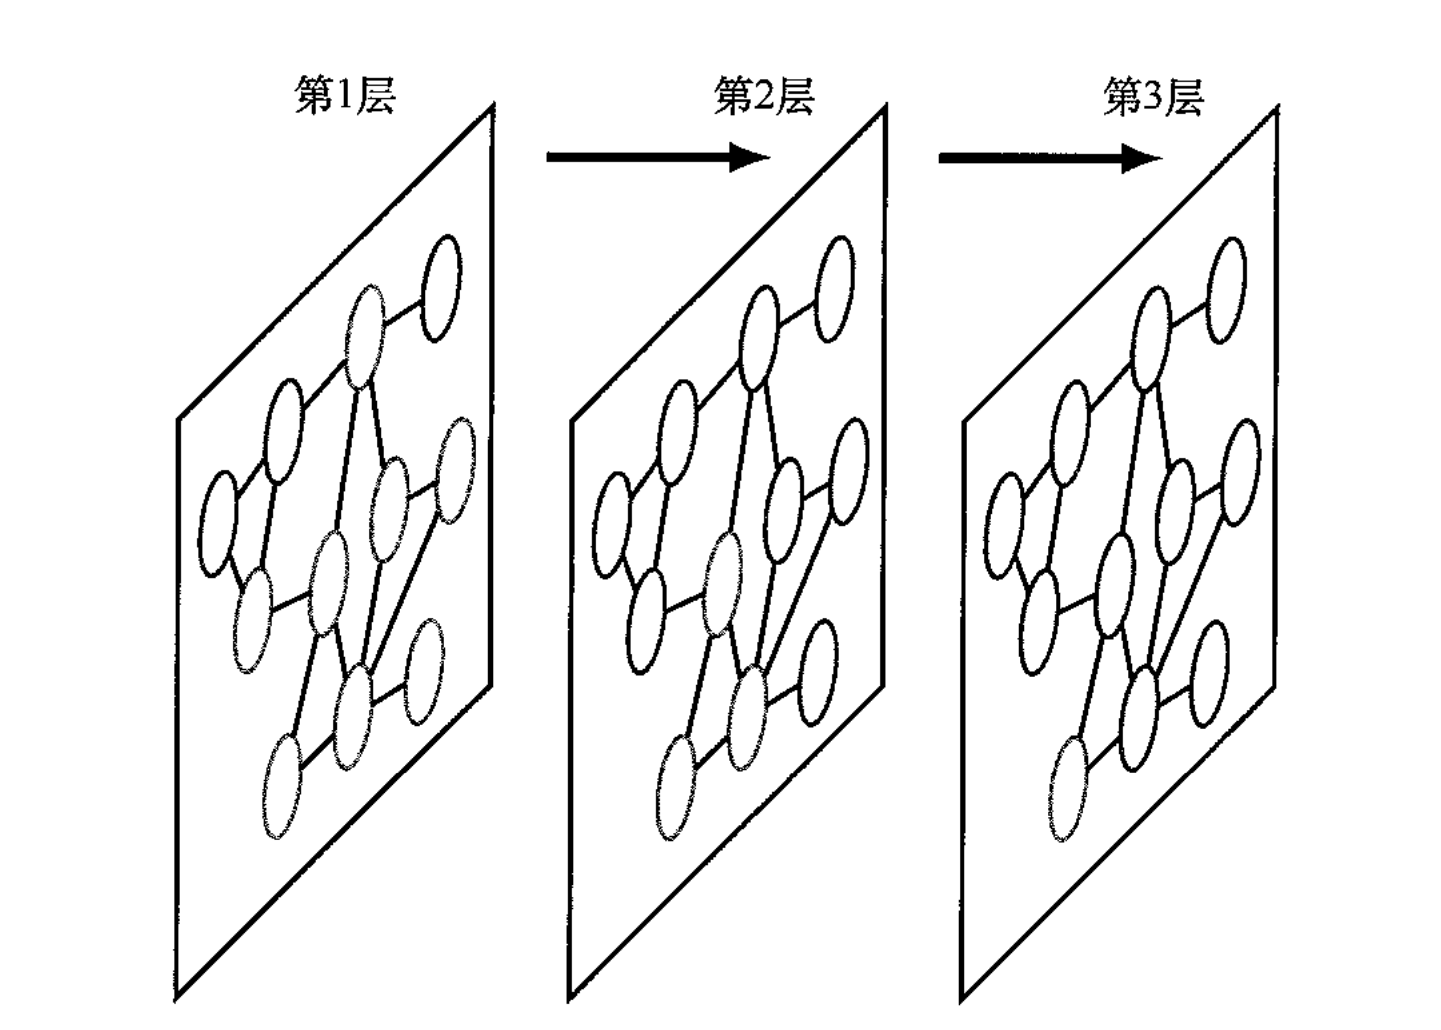
\includegraphics[width=0.62\textwidth]{ch13-fig13.4-receptive.png}
  \caption{通过图神经网络连续层的信息流示意图。在第 3 层中，只有一个节点以红色突出显示。该节点从前一层的两个邻居节点接收信息，而这两个邻居节点又从第 1 层的邻居节点接收信息。就像用于图像的卷积神经网络一样，有效感受野——对应于显示为红色的节点数量——会随着处理层数的增加而扩大}
  \label{figure:ch13-感受野}
\end{figure}

迄今为止我们所讨论的聚合算子都没有可学习参数。如果我们在组合邻居节点的嵌入向量之前，先使用一个多层神经网络（用 $\operatorname{MLP}_\phi$ 表示）对每个嵌入向量进行变换，那么我们就可以引入这样的参数，其中 MLP 代表“多层感知机”，其下标 $\phi$ 表示网络的参数。只要网络具有跨节点共享的结构和参数值，那么这个聚合算子就是排列不变的。

\begin{definition}[深度集合聚合算子]\label{definition:ch13-深度集合聚合}
还可以使用另一个参数为 $\theta$ 的神经网络 $\operatorname{MLP}_\theta$ 来转换组合向量，从而得到如下一般性的聚合操作：
\begin{align}
\operatorname{Aggregate}\!\left(\{\bm{h}_m^{(l)}:m\in\mathcal{N}(n)\}\right)=\operatorname{MLP}_\theta\!\left(\sum_{m\in\mathcal{N}(n)}\operatorname{MLP}_\phi(\bm{h}_m^{(l)})\right),
\label{align:ch13-深度集合聚合}
\end{align}
其中 $\operatorname{MLP}_\phi$ 和 $\operatorname{MLP}_\theta$ 在网络第 $l$ 层是共享的。由于 MLP 的灵活性，\eqref{align:ch13-深度集合聚合}定义的转换代表了任何置换不变函数的通用逼近器，该函数能将一组嵌入映射到单个嵌入（Zaheer et al., 2017）。注意，这里的求和操作可以替换为其他的置换不变函数，例如平均值，逐元素取最大值或最小值。
\end{definition}

% SUPPLEMENT: parent=definition:ch13-深度集合聚合; kind=motivation; location=紧随其后的 remark（重构新增）
\begin{remark}（重构新增）
\eqref{align:ch13-深度集合聚合}的结构可以概括为“逐元素变换—求和—再变换”，它是“先聚合、再更新”框架中最常用的一种聚合算子。把 $\operatorname{MLP}_\phi$ 放在求和之前的理由是可以逐节点独立计算，从而可以并行；把 $\operatorname{MLP}_\theta$ 放在求和之后的理由是它需要看到整个邻域的信息，而求和已经把邻域压成一个定长向量。两个 MLP 在同一层的所有节点、所有位置之间共享参数，这既是置换等变性的来源，也是参数量与节点数无关的原因。\par
定义中“求和可以替换为平均值、逐元素最大值或最小值”这句话有条件：替换后的函数仍必须是置换不变的。求和、平均、逐元素最大/最小都满足这一点，而按邻居编号加权求和、把邻居向量按序拼接都不满足。另外，用最大值替换求和会改变算子对邻居个数的敏感性（最大值只看“最强的那个邻居”），表达能力与稳定性都随之变化，这不是无关紧要的实现细节。\par
定义把“通用逼近”作为一句引用的结论写在正文里。它比“置换不变”强得多：置换不变只说明函数不区分顺序，通用逼近说明任何连续置换不变函数都能被这一族算子逼近。完整的证明属于文献而不是本章，下面的\cref{proposition:ch13-深度集合置换不变性}只证明其中可以直接验证的一半。
\end{remark}

\begin{proposition}[深度集合聚合的置换不变性]\label{proposition:ch13-深度集合置换不变性}
设 $\bm{h}_1,\cdots,\bm{h}_K$ 为某节点邻居的嵌入向量，$\sigma$ 为 $\{1,\cdots,K\}$ 的任意置换。定义
\begin{align*}
F(\{\bm{h}_1,\cdots,\bm{h}_K\})=\operatorname{MLP}_\theta\!\left(\sum_{k=1}^{K}\operatorname{MLP}_\phi(\bm{h}_k)\right),
\end{align*}
则 $F(\{\bm{h}_{\sigma(1)},\cdots,\bm{h}_{\sigma(K)}\})=F(\{\bm{h}_1,\cdots,\bm{h}_K\})$，即\eqref{align:ch13-深度集合聚合}的聚合算子与邻居的排序无关。
\end{proposition}

\begin{proof}（重构新增）
设 $\{\bm{h}'_1,\cdots,\bm{h}'_K\}$ 是 $\{\bm{h}_1,\cdots,\bm{h}_K\}$ 的一个重排，即存在置换 $\sigma$ 使 $\bm{h}'_k=\bm{h}_{\sigma(k)}$。则内层求和满足
\begin{align*}
\sum_{k=1}^{K}\operatorname{MLP}_\phi(\bm{h}'_k)=\sum_{k=1}^{K}\operatorname{MLP}_\phi(\bm{h}_{\sigma(k)})=\sum_{k'=1}^{K}\operatorname{MLP}_\phi(\bm{h}_{k'}),
\end{align*}
其中第二个等号是有限和的重指标（$\sigma$ 是双射，遍历 $k$ 等价于遍历 $k'=\sigma(k)$）。这里用到 $\operatorname{MLP}_\phi$ 逐元素作用、与 $\bm{h}$ 的下标无关这一事实。由于内层求和的结果完全相同，再经过同一个 $\operatorname{MLP}_\theta$ 得到的输出也相同，故 $F$ 对邻居的任意重排不变。证毕。
\end{proof}

% SUPPLEMENT: parent=proposition:ch13-深度集合置换不变性; kind=motivation; location=紧随其后的 remark（重构新增）
\begin{remark}（重构新增）
命题的证明只有一步，但它的条件值得逐条核对。第一，$\operatorname{MLP}_\phi$ 必须对所有邻居使用同一组参数；若每个邻居有自己的 $\operatorname{MLP}$，重排会改变“哪个网络作用在哪个向量上”，结论立刻失效。第二，内层必须是对全部邻居的求和（或平均、最大），而不能是带位置权重的加权和。第三，$\operatorname{MLP}_\theta$ 只作用于求和结果这一个向量，因此它看不到邻居的顺序。\par
反向的问题是这条命题回答不了的：满足置换不变的函数很多，为什么偏偏选“变换—求和—变换”这一族？Zaheer et al. (2017) 的结论给出了回答：在温和的连续性条件下，任何置换不变的连续函数都可以写成 $\rho\left(\sum_k\phi(\bm{h}_k)\right)$ 的形式，而 $\rho$ 与 $\phi$ 可以用 MLP 逼近。原书引用这一结论而未加证明，它属于本章范围之外的逼近论结果；本注记只说明它的地位，不把它当作已证事实使用。\par
最后，当图没有边时 $\mathcal{N}(n)$ 只含其他所有节点，\eqref{align:ch13-深度集合聚合}就退化为作用在无结构集合上的算子，这解释了原书所说的“深度集合”（deep set）是图神经网络的特例：图神经网络严格包含深度集合，反之不成立。
\end{remark}

如果我们考虑一个没有边的图，它就退化成了一个简单的无结构节点集合，这时的图神经网络就成为一个特例。在这种情况下，如果我们对集合中的每个向量 $\bm{h}_n^{(l)}$ 应用\eqref{align:ch13-深度集合聚合}，其中求和是在除 $\bm{h}_n^{(l)}$ 外的所有其他向量上进行的，那么我们就有了一个关于无结构变量集合［称为深度集合（deep set）］的学习函数的通用框架。

\subsection{更新算子}\label{subsection:ch13-更新算子}

在选择了合适的聚合算子之后，我们同样需要决定更新算子的形式。类似于 CNN 的公式\eqref{align:ch13-图卷积滤波}，一种简单的更新算子形式如下：
\begin{align}
\operatorname{Update}\!\left(\bm{h}_n^{(l)},\bm{z}_n^{(l)}\right)=f\!\left(\bm{W}_{\mathrm{self}}\bm{h}_n^{(l)}+\bm{W}_{\mathrm{neigh}}\bm{z}_n^{(l)}+\bm{b}\right),
\label{align:ch13-更新算子}
\end{align}
其中 $f(\cdot)$ 是一个非线性激活函数，例如可以逐元素应用到向量参数上的 ReLU 函数；$\bm{W}_{\mathrm{self}}$ 和 $\bm{W}_{\mathrm{neigh}}$ 是可学习权重；$\bm{b}$ 是偏置；$\bm{z}_n^{(l)}$ 由\eqref{align:ch13-聚合定义}定义。

\begin{definition}[更新算子]\label{definition:ch13-更新算子}
若选择简单的求和\eqref{align:ch13-求和聚合}作为聚合函数，并且在节点及其邻居节点之间共享相同的权重矩阵，使得 $\bm{W}_{\mathrm{self}}=\bm{W}_{\mathrm{neigh}}$，就能得到如下特别简单的更新算子形式：
\begin{align}
\bm{h}_n^{(l+1)}=\operatorname{Update}\!\left(\bm{h}_n^{(l)},\bm{z}_n^{(l)}\right)=f\!\left(\bm{W}_{\mathrm{neigh}}\sum_{m\in\mathcal{N}(n),n}\bm{h}_m^{(l)}+\bm{b}\right).
\label{align:ch13-简单更新}
\end{align}
\end{definition}

% SUPPLEMENT: parent=definition:ch13-更新算子; kind=motivation; location=紧随其后的 remark（重构新增）
\begin{remark}（重构新增）
\eqref{align:ch13-更新算子}与\eqref{align:ch13-简单更新}的差别不只是“少了一个矩阵”。前者对“节点自身”和“邻居聚合”使用两个不同的线性映射，因而能够表达“我”与“我的邻域”在语义上的不同角色；后者令两者共用 $\bm{W}_{\mathrm{neigh}}$，相当于把节点自身也当作一个邻居，于是\eqref{align:ch13-简单更新}中的求和写成了 $\sum_{m\in\mathcal{N}(n),n}$——这个逗号加 $n$ 正是“给图补上自环”的记号版本。\par
\eqref{align:ch13-更新算子}中的三个参数各有分工：$\bm{W}_{\mathrm{self}}$ 决定如何保留节点自身的信息，$\bm{W}_{\mathrm{neigh}}$ 决定如何吸收邻域信息，$\bm{b}$ 提供一个与节点无关的平移。若去掉 $\bm{W}_{\mathrm{self}}$ 这一项，节点在更新后会“忘记”自己原来的特征，多层之后所有节点的表示只由结构决定；若去掉 $\bm{W}_{\mathrm{neigh}}$，图结构就完全不起作用。\par
两个矩阵的维数必须匹配：$\bm{h}_n^{(l)}\in\mathbb{R}^{D_l}$、$\bm{h}_n^{(l+1)}\in\mathbb{R}^{D_{l+1}}$ 时，$\bm{W}_{\mathrm{self}},\bm{W}_{\mathrm{neigh}}\in\mathbb{R}^{D_{l+1}\times D_l}$、$\bm{b}\in\mathbb{R}^{D_{l+1}}$。这与原书未显式写出维数的做法一致，但在实现时必须核对。
\end{remark}

消息传递算法通常通过设置 $\bm{h}_n^{(0)}=\bm{x}_n$ 来初始化。然而，有时我们可能希望每个节点都有一个内部表示向量，其维度不同于 $\bm{x}_n$ 的维度。这样的表示可以通过用额外的零填充节点向量 $\bm{x}_n$（以达到更高的维度），或者简单地使用可学习的线性变换将节点向量转换到所需维度的空间来初始化。当节点没有与之关联的数据变量时，一种替代的初始化形式是使用一个标记了每个节点度数（即邻居节点数量）的独热向量。

总的来说，我们可以将图神经网络表示为一系列连续变换节点嵌入的层。如果我们将这些嵌入分组到一个矩阵 $\bm{H}$ 中，其第 $n$ 行是向量 $\bm{h}_n^{\mathsf T}$，并初始化为数据矩阵 $\bm{X}$，则可以将这些连续的变换写成以下形式：

\begin{definition}[图网络的层叠表示]\label{definition:ch13-图网络层叠}
\begin{align}
\bm{H}^{(1)}&=\bm{F}\!\left(\bm{X},\bm{A},\bm{W}^{(1)}\right)\nonumber\\
\bm{H}^{(2)}&=\bm{F}\!\left(\bm{H}^{(1)},\bm{A},\bm{W}^{(2)}\right)\nonumber\\
&\vdots\nonumber\\
\bm{H}^{(L)}&=\bm{F}\!\left(\bm{H}^{(L-1)},\bm{A},\bm{W}^{(L)}\right),
\label{align:ch13-层叠}
\end{align}
其中 $\bm{A}$ 是邻接矩阵，$\bm{W}^{(l)}$ 表示网络第 $l$ 层中全部权重和偏置的集合。
\end{definition}

% SUPPLEMENT: parent=definition:ch13-图网络层叠; kind=motivation; location=紧随其后的 remark（重构新增）
\begin{remark}（重构新增）
\eqref{align:ch13-层叠}把“深度”写成了同一个算子 $\bm{F}$ 的反复复合，其中每一层只更换参数集合 $\bm{W}^{(l)}$，图结构 $\bm{A}$ 在所有层中保持不变。这个写法有两个直接好处：一是它把“层数”与“图的规模”彻底解耦，$L$ 是网络的超参数而 $N$ 由数据决定；二是它为归纳证明提供了合适的形式——只要证明单层 $\bm{F}$ 与置换矩阵可交换，复合的等变性就自动成立（\cref{theorem:ch13-图网络等变性}）。\par
注意 $\bm{F}$ 的第二个自变量始终是同一个 $\bm{A}$，而不是 $\bm{A}^{(l)}$。有些架构会随层改变图的连接（例如池化后粗化图），那就不再是\eqref{align:ch13-层叠}的形式，需要另作分析。另外，$\bm{W}^{(l)}$ 逐层不同是默认设定；原书也提到参数可以跨层共享，那相当于令所有 $\bm{W}^{(l)}$ 相等，此时 $\bm{F}$ 的反复复合就是一个迭代映射，其不动点与过度平滑现象直接相关（\cref{subsection:ch13-过度平滑}）。
\end{remark}

在置换矩阵 $\bm{P}$ 定义的节点重新排序下，第 $l$ 层计算的节点嵌入的变换是等变的：
\begin{align}
\bm{P}\bm{H}^{(l)}=\bm{F}\!\left(\bm{P}\bm{H}^{(l-1)},\bm{P}\bm{A}\bm{P}^{\mathsf T},\bm{W}^{(l)}\right).
\label{align:ch13-层等变性}
\end{align}

\begin{theorem}[图神经网络的置换等变性]\label{theorem:ch13-图网络等变性}
设单层变换 $\bm{F}$ 由\eqref{align:ch13-聚合定义}与\eqref{align:ch13-更新定义}给出，其中聚合算子对邻居的排序不变、更新算子逐节点作用且参数在所有节点间共享。若对某一层 $l$ 有\eqref{align:ch13-层等变性}，则对由\eqref{align:ch13-层叠}定义的整个网络，
\begin{align*}
\bm{P}\bm{H}^{(L)}=\bm{F}\!\left(\bm{P}\bm{H}^{(L-1)},\bm{P}\bm{A}\bm{P}^{\mathsf T},\bm{W}^{(L)}\right)
\end{align*}
对任意置换矩阵 $\bm{P}$ 成立；换言之，整个网络计算出一个等变的转换。
\end{theorem}

\begin{proof}（重构新增）
对层数 $l$ 作归纳。归纳假设为：当输入数据被 $\bm{P}$ 重排，即 $\widetilde{\bm{X}}=\bm{P}\bm{X}$、$\widetilde{\bm{A}}=\bm{P}\bm{A}\bm{P}^{\mathsf T}$ 时，第 $l$ 层的嵌入满足 $\widetilde{\bm{H}}^{(l)}=\bm{P}\bm{H}^{(l)}$。\par
奠基 $l=0$：由初始化 $\bm{H}^{(0)}=\bm{X}$ 及\eqref{align:ch13-数据矩阵置换}，$\widetilde{\bm{H}}^{(0)}=\widetilde{\bm{X}}=\bm{P}\bm{X}=\bm{P}\bm{H}^{(0)}$。
归纳步：设 $\widetilde{\bm{H}}^{(l-1)}=\bm{P}\bm{H}^{(l-1)}$。由\eqref{align:ch13-层叠}，$\widetilde{\bm{H}}^{(l)}=\bm{F}(\widetilde{\bm{H}}^{(l-1)},\widetilde{\bm{A}},\bm{W}^{(l)})=\bm{F}(\bm{P}\bm{H}^{(l-1)},\bm{P}\bm{A}\bm{P}^{\mathsf T},\bm{W}^{(l)})$。由单层等变性\eqref{align:ch13-层等变性}，右端等于 $\bm{P}\bm{F}(\bm{H}^{(l-1)},\bm{A},\bm{W}^{(l)})=\bm{P}\bm{H}^{(l)}$，归纳步完成。
还需说明\eqref{align:ch13-层等变性}本身为什么成立，否则归纳是空的。设 $\widetilde{\bm{H}}=\bm{P}\bm{H}$，即 $\widetilde{\bm{h}}_n=\bm{h}_{\pi^{-1}(n)}$，并记 $\widetilde{\mathcal{N}}(n)=\pi(\mathcal{N}(\pi^{-1}(n)))$。聚合阶段：
\begin{align*}
\widetilde{\bm{z}}_n&=\operatorname{Aggregate}\left(\{\widetilde{\bm{h}}_m:m\in\widetilde{\mathcal{N}}(n)\}\right)\\
&=\operatorname{Aggregate}\left(\{\bm{h}_{m'}:m'\in\mathcal{N}(\pi^{-1}(n))\}\right)=\bm{z}_{\pi^{-1}(n)},
\end{align*}
第一个等号用 $\widetilde{\bm{A}}=\bm{P}\bm{A}\bm{P}^{\mathsf T}$ 所刻画的邻接关系（$\widetilde A_{nm}=A_{\pi^{-1}(n)\pi^{-1}(m)}$），第二个等号只是重指标 $m'=\pi^{-1}(m)$，最后一个等号用聚合对排序不变这一假设。更新阶段：
\begin{align*}
\widetilde{\bm{h}}_n^{(l+1)}&=\operatorname{Update}\left(\widetilde{\bm{h}}_n,\widetilde{\bm{z}}_n\right)\\
&=\operatorname{Update}\left(\bm{h}_{\pi^{-1}(n)},\bm{z}_{\pi^{-1}(n)}\right)=\bm{h}_{\pi^{-1}(n)}^{(l+1)},
\end{align*}
其中第二个等号用归纳假设与上一式，第三个等号用更新算子逐节点作用且参数共享。合并得 $\widetilde{\bm{H}}^{(l)}=\bm{P}\bm{H}^{(l)}$，即\eqref{align:ch13-层等变性}。取 $l=L$ 即得定理结论。证毕。
\end{proof}

% SUPPLEMENT: parent=theorem:ch13-图网络等变性; kind=motivation; location=紧随其后的 remark（重构新增）
\begin{remark}（重构新增）
这个定理是本章的中心结论，它把“图神经网络尊重节点编号的任意性”从一句设计口号变成了对任意层数的严格断言。证明的结构值得记住：等变性不是逐层“偶然成立”的，而是由单层性质加归纳传递的，因此只要单层满足\eqref{align:ch13-层等变性}，无论堆多少层都不会破坏它。这也解释了\cref{section:ch13-神经信息传递}开头那句“如果网络的每一层都在节点重新排序后保持等变性，那么多层叠加后的网络也将保持等变性”。\par
定理对聚合算子与更新算子的要求是充分的，但不是必要的：某些并不逐层等变的架构（例如在中间层做全局池化）仍可能给出不变的整体输出。定理也不涉及数值稳定性、表达能力或泛化，它只断言对称性。\par
还要注意，等变的是 $\bm{H}^{(L)}$ 这一整块节点嵌入，而不是某个图级标量。若要得到图级预测，必须在 $\bm{H}^{(L)}$ 之后接一个置换不变的读出函数，否则输出会随编号改变——这正是下一小节与\cref{subsection:ch13-图分类}的分工。
\end{remark}

\subsection{节点分类}\label{subsection:ch13-节点分类}

图神经网络可以看作一系列层，其中的每一层都将一组节点嵌入向量 $\{\bm{h}_n^{(l)}\}$ 转换成同样大小和维度的新向量集合 $\{\bm{h}_n^{(l+1)}\}$。在网络的最后一个卷积层之后，我们需要得到预测结果，以便定义一个用于训练的损失函数，以及使用训练好的网络对新数据进行预测。

考虑对图中节点分类的任务，这是图神经网络最常见的用途之一。我们可以定义一个输出层，有时称为读出层（readout layer），该层为每个节点计算一个与 $C$ 个分类相对应的 softmax 函数。

\begin{definition}[读出层与节点分类损失]\label{definition:ch13-读出层}
读出层的输出由 softmax 函数给出，形式如下：
\begin{align}
y_{ni}=\frac{\exp\!\left(\bm{w}_i^{\mathsf T}\bm{h}_n^{(L)}\right)}{\sum_j\exp\!\left(\bm{w}_j^{\mathsf T}\bm{h}_n^{(L)}\right)},
\label{align:ch13-节点softmax}
\end{align}
其中 $\{\bm{w}_i\}$ 是一组可学习的权重向量，$i=1,\cdots,C$。我们可以将损失函数定义为所有节点和所有类别的交叉熵损失之和：
\begin{align}
\mathcal{L}=-\sum_{n\in\mathcal{V}_{\mathrm{train}}}\sum_{i=1}^{C}t_{ni}\ln y_{ni},
\label{align:ch13-节点交叉熵}
\end{align}
其中 $t_{ni}$ 是目标值，每个 $n$ 值都有一个独热编码。
\end{definition}

% SUPPLEMENT: parent=definition:ch13-读出层; kind=motivation; location=紧随其后的 remark（重构新增）
\begin{remark}（重构新增）
\eqref{align:ch13-节点softmax}与普通的 softmax 回归形式完全相同，唯一的区别在于输入 $\bm{h}_n^{(L)}$ 已经通过 $L$ 层消息传递融合了邻域信息。因此“图神经网络做节点分类”并没有引入新的输出层，它只是把特征提取换成了尊重图结构的那一种。\par
\eqref{align:ch13-节点交叉熵}中的求和范围是 $\mathcal{V}_{\mathrm{train}}$ 而不是全部节点，这是节点分类与普通分类的关键差别：图是半监督设定的载体，未标注节点仍然参与消息传递（它们出现在\eqref{align:ch13-聚合定义}的邻居集合中），只是不进入损失。这一点在下一段的三类节点划分中被明确区分。\par
$t_{ni}$ 取独热编码是一个约定，它使\eqref{align:ch13-节点交叉熵}简化为 $-\sum_{n}\ln y_{n,t_n}$，其中 $t_n$ 是节点 $n$ 的类别。若标签有软分配（例如标注者的分歧），则保留一般的 $t_{ni}$ 即可。
\end{remark}

\begin{proposition}[节点分类损失的置换不变性]\label{proposition:ch13-节点分类损失不变性}
设 $y_{ni}$ 由\eqref{align:ch13-节点softmax}给出，$\mathcal{L}$ 由\eqref{align:ch13-节点交叉熵}给出，$t_{ni}$ 随节点一同重排。则对任意置换矩阵 $\bm{P}$，有 $\mathcal{L}(\widetilde{\bm{H}}^{(L)},\widetilde{\bm{t}})=\mathcal{L}(\bm{H}^{(L)},\bm{t})$。
\end{proposition}

\begin{proof}（重构新增）
由\cref{theorem:ch13-图网络等变性}，$\widetilde{\bm{h}}_n^{(L)}=\bm{h}_{\pi^{-1}(n)}^{(L)}$。由于权重向量 $\bm{w}_i$ 在所有节点间共享，\eqref{align:ch13-节点softmax}对每个节点逐点计算，故
\begin{align*}
\widetilde{y}_{ni}&=\frac{\exp(\bm{w}_i^{\mathsf T}\widetilde{\bm{h}}_n^{(L)})}{\sum_j\exp(\bm{w}_j^{\mathsf T}\widetilde{\bm{h}}_n^{(L)})}\\
&=\frac{\exp(\bm{w}_i^{\mathsf T}\bm{h}_{\pi^{-1}(n)}^{(L)})}{\sum_j\exp(\bm{w}_j^{\mathsf T}\bm{h}_{\pi^{-1}(n)}^{(L)})}=y_{\pi^{-1}(n),i},
\end{align*}
即输出随节点一同等变。又 $t_{ni}$ 随节点重排，$\widetilde{t}_{ni}=t_{\pi^{-1}(n),i}$，于是每一项 $\widetilde{t}_{ni}\ln\widetilde{y}_{ni}=t_{\pi^{-1}(n),i}\ln y_{\pi^{-1}(n),i}$。对 $n\in\mathcal{V}_{\mathrm{train}}$ 求和时作重指标 $n'=\pi^{-1}(n)$，训练集 $\mathcal{V}_{\mathrm{train}}$ 也随节点一同重排为 $\widetilde{\mathcal{V}}_{\mathrm{train}}=\pi(\mathcal{V}_{\mathrm{train}})$，故和值不变：$\mathcal{L}(\widetilde{\bm{H}}^{(L)},\widetilde{\bm{t}})=\mathcal{L}(\bm{H}^{(L)},\bm{t})$。证毕。
\end{proof}

% SUPPLEMENT: parent=proposition:ch13-节点分类损失不变性; kind=motivation; location=紧随其后的 remark（重构新增）
\begin{remark}（重构新增）
这条命题说明了“损失不变”是怎么来的：等变的输出乘上同样等变的目标，再对节点求和，重排只是把求和项重新排列。三个条件都不能少——$\bm{w}_i$ 必须共享（否则 $\widetilde{y}$ 不等于 $y$ 的重排）、目标必须随节点重排（否则求和项被错配）、求和必须遍历同一批节点（否则重排会改变训练集）。\par
如果目标是在输出处预测连续值而非类别，则把\eqref{align:ch13-节点softmax}换成线性变换、把\eqref{align:ch13-节点交叉熵}换成平方和误差即可，命题的论证逐字不变，因为只用到“逐节点计算 + 共享参数 + 对节点求和”这三点。
\end{remark}

式\eqref{align:ch13-节点交叉熵}中对 $n$ 的求和是在用于训练的节点子集 $\mathcal{V}_{\mathrm{train}}$ 上进行的。我们需要区分以下 3 种类型的节点。

\begin{enumerate}[label=（\arabic*）]
\item 节点子集 $\mathcal{V}_{\mathrm{train}}$ 中的节点是有标签的，既参与图神经网络的消息传递操作，也用于计算训练的损失函数。
\item 可能还有一个名为 $\mathcal{V}_{\mathrm{trans}}$ 的节点子集，里面是未标记的直推式（transductive）节点并且不参与用于训练的损失函数的计算。然而，它们仍然参与训练和推理阶段的消息传递，它们的标签可能会作为推理过程的一部分被预测。
\item 剩余的节点标记为 $\mathcal{V}_{\mathrm{induct}}$，是一组归纳节点，它们不用于计算损失函数，并且这些节点及其关联的边在训练阶段不参与消息传递。然而，它们在推理阶段参与消息传递，它们的标签预测为推理的结果。
\end{enumerate}

\begin{definition}[归纳学习与直推式学习]\label{definition:ch13-归纳与直推学习}
如果没有直推式节点，即测试节点（及其关联的边）在训练阶段不可用，那么通常将这种训练称为归纳学习（inductive learning），这可以视为一种监督学习（supervised learning）的形式。然而，如果存在直推式节点，则称这种训练为直推式学习（transductive learning），这可以视为半监督（semi-supervised）学习的一种形式。
\end{definition}

% SUPPLEMENT: parent=definition:ch13-归纳与直推学习; kind=motivation; location=紧随其后的 remark（重构新增）
\begin{remark}（重构新增）
这三类节点的划分不是术语游戏，它决定了训练时哪些边可以出现在计算图中。$\mathcal{V}_{\mathrm{train}}$ 与 $\mathcal{V}_{\mathrm{trans}}$ 的节点在训练阶段参与消息传递，因此它们的特征会通过邻居影响有标签节点的嵌入；$\mathcal{V}_{\mathrm{induct}}$ 的节点及其边在训练阶段被完全移出，因此模型在训练时从未见过它们。\par
这个区别对应两种不同的泛化问题。直推式学习回答的是“在这张已经给定的图上，未标注节点的标签是什么”，模型可以（也必然）利用测试节点的结构位置；归纳学习回答的是“对一张训练时从未出现过的新图，如何预测”，因此要求模型对任意图都能前向计算。分子性质预测属于后者，社交网络中的用户分类通常属于前者。\par
从工程角度看，直推式的代价是模型与特定图绑定，图一变就必须重新训练；归纳式的代价是必须让所有参数与 $N$ 无关，而这正好由参数共享（\cref{theorem:ch13-图网络等变性}）保证。
\end{remark}

\subsection{边分类}\label{subsection:ch13-边分类}

在某些应用中，我们希望对图的边而不是节点进行预测。一种常见的边分类任务是边补全。在这种任务中，目标是确定两个节点之间是否应该存在一条边。给定一组节点嵌入，可以使用嵌入向量之间的点积，通过逻辑斯谛 sigmoid 函数定义两个节点 $n$ 和 $m$ 之间存在边的概率 $p(n,m)$。

\begin{definition}[边存在概率]\label{definition:ch13-边存在概率}
两个节点 $n$ 和 $m$ 之间存在边的概率定义为
\begin{align}
p(n,m)=\sigma\!\left(\bm{h}_n^{\mathsf T}\bm{h}_m\right),
\label{align:ch13-边概率}
\end{align}
其中 $\sigma(\cdot)$ 是逻辑斯谛 sigmoid 函数，$\bm{h}_n,\bm{h}_m$ 为最终的节点嵌入。
\end{definition}

% SUPPLEMENT: parent=definition:ch13-边存在概率; kind=motivation; location=紧随其后的 remark（重构新增）
\begin{remark}（重构新增）
用内积构造边得分是“嵌入空间几何”的直接体现：两个节点的嵌入越同向、模越长，内积越大，判定存在边的概率越高。它的一个好处是对称——$p(n,m)=p(m,n)$，与本章的无向图假设一致；若图是有向的，就需要把 $\bm{h}_n^{\mathsf T}\bm{h}_m$ 换成 $\bm{h}_n^{\mathsf T}\bm{W}\bm{h}_m$ 之类的不对称形式。\par
\eqref{align:ch13-边概率}对节点重排是等变的：重排只会把 $p(n,m)$ 换成 $p(\pi(n),\pi(m))$，而不会改变任何一对节点之间的数值，因此以边为单位计算损失时整体不变。这一点与\cref{proposition:ch13-节点分类损失不变性}同理，不再单列命题。\par
注意 $p(n,m)$ 只用了两个端点的嵌入，没有显式使用边的特征。若边本身带有观测数据，应当把它们并入 $\bm{h}$ 或改用\cref{definition:ch13-边嵌入消息传递}中的边嵌入。
\end{remark}

\begin{example}[ 社交网络中的边预测]\label{example:ch13-社交网络边预测}
一个典型的应用实例是，预测社交网络中任意两个用户是否拥有共同的兴趣爱好，并愿意建立联系。
\end{example}

\subsection{图分类}\label{subsection:ch13-图分类}

在图神经网络的某些应用中，我们要在给定一组带标签的训练图 $\mathcal{G}_1,\cdots,\mathcal{G}_N$ 的情况下，预测新图的属性。这要求我们以不依赖于任意节点排序的方式组合最终层的嵌入向量，从而确保输出的预测结果与节点的排序无关。这任务有点像聚合函数，只不过这里考虑的是图中所有节点，而不仅仅是单个节点的邻域集。

\begin{definition}[图级读出函数]\label{definition:ch13-图级读出}
最简单的方法是对节点嵌入向量进行求和：
\begin{align}
y=f\!\left(\sum_{n\in\mathcal{V}}\bm{h}_n^{(L)}\right),
\label{align:ch13-图级读出}
\end{align}
其中，函数 $f$ 可能包含可学习参数，如线性变换或神经网络。也可以使用其他不变的聚合函数，例如平均值、逐元素的最小值或最大值。
\end{definition}

% SUPPLEMENT: parent=definition:ch13-图级读出; kind=motivation; location=紧随其后的 remark（重构新增）
\begin{remark}（重构新增）
读出函数是“等变 → 不变”的转换器：$\bm{H}^{(L)}$ 是等变的，对它做一次置换不变的归约就得到与节点编号无关的 $y$。\eqref{align:ch13-图级读出}选的是求和，于是 $y$ 只依赖全部节点嵌入的多重集合，而不依赖它们分别属于哪个节点——这正是图级预测需要的语义。\par
求和与平均在这里的差别比在聚合算子中更实质：求和使 $y$ 随图的规模（节点数）增长，因此同一个模型在不同大小的图上给出的 $y$ 量级不同；平均则消除了节点数的影响。分子性质预测通常用求和或平均都能工作，但若训练集与测试集的分子大小分布差异很大，平均更稳妥。逐元素最大值只保留每个维度上最突出的节点，适合“是否存在某种子结构”这类问题。\par
$f$ 中是否含可学习参数不影响不变性，因为 $f$ 作用在已经归约好的单个向量上，看不到节点顺序。
\end{remark}

\begin{example}[ 候选药物分子的图分类]\label{example:ch13-药物分子图分类}
对于分类问题，例如将候选药物分子标记为有毒或安全，通常采用交叉熵损失函数；而对于回归问题，例如预测候选药物分子的溶解度，则通常采用平方误差损失函数。图级别的预测对应于归纳任务，因为必须有不同的图集合用于训练和推理。
\end{example}

\end{document}
